\documentclass[conference]{IEEEtran-ModifiedForMVIP}
% این فایل از روی نمونه‌ فایل ارائه شده برای کنفرانس مهندسی برق ایران ICEE 
% برای کنفرانس بینایی ماشین و پردازش تصویر ایران به‌روزرسانی شده است.
% فایل منبع و فایلهای ضمیمه‌ی آن با تغییر فایلهایی که توسط آقای دکتر محمود امین طوسی (دانشگاه
% حکیم سبزواری، http://profs.hsu.ac.ir/mamintoosi) در سایت www.parsilatex.com قرار داده 
% شده بودند به دست آمده است. این تغییرات توسط دکتر مسعود بابایی‌زاده داده شده است. 
% البته فایل IEEEtran-ModifiedForICEE.cls در اینجا، 
% اصلاح شده فایل آقای دکتر امین طوسی نیست و مستقیما با دستکاری
% در فایل IEEEtran.cls توسط مسعود بابایی زاده ایجاد شده است.
% برای کنفرانس بینایی ماشین و پردازش تصویر ایران، فایل IEEEtran-ModifiedForICEE.cls 
% با نام IEEEtran-ModifiedForMVIP.cls  تغییر داده شده است.

% مقاله اصلی که این فایل از تغییر فایل آن به دست آمده است، در هفدهمین کنفرانس مهندسی برق 
% ایران در اردیبهشت ۸۸ ارائه شده بوده است.

% شما می‌توانید از این فایل به عنوان یک الگو برای مقالات خود استفاده نمایید.

% برای پردازش پس از یکبار استفاده از xelatex با استفاده از دستور زیر لیست مراجع را تولید نمایید:
% bibtex MVIP_FA_LaTeX_SamplePaper
% و سپس دوبار استفاده از xelatex. 

%%%% فراخوانی پکیج‌های مورد نیاز کاربر %%%%%%%%%%%%%%%%%%%%%%%%%%%%%%%%%%%%%%%%%%%%%%%%%%
\usepackage{listings}
\usepackage{setspace}
\usepackage{subfigure}
\usepackage{algorithm}
\usepackage{algorithmic}
\usepackage{graphicx}
\usepackage{amsmath}
\usepackage{amssymb}
\usepackage{booktabs}
\usepackage{pdfpages}
%\usepackage[colorlinks, citecolor=blue]{hyperref}

%%%%%%%%%%%%%%%%%%%%%%%%%%%%%%%%%%%%%%%%%%%%%%%%%%%%%%%%%%%%%%%%%%%%%%%%%%%%%%%%%%%%%%%%
%%%% فراخوانی تنظیمات مورد نیاز کنفرانس مهندسی برق ایران و پکیج زی‌پرشین %%%%%%%%%%%%%%%%
% این فایل از روی نمونه‌ فایل ارائه شده برای کنفرانس مهندسی برق ایران ICEE برای کنفرانس بینایی ماشین و پردازش تصویر ایران به‌روزرسانی شده است.
% این فایل شامل تنظیماتی است که قبل از لود شدن پکیج زی‌پرشین باید انجام شوند.
% نویسنده: مسعود بابایی‌زاده
% نسخه 1.0.0
% تاریخ: ۵ مهرماه ۱۳۹۳
%%%%%%%%%%%%%%%%%%%%%%%%%%%%%%%%%%%%%%%%%%
% Start of Page Setup:
\usepackage[top=25mm, bottom=25mm, left=20mm, right=20mm]{geometry}
\setlength{\columnwidth}{82mm}
\setlength{\columnsep}{6mm}
% End of Page Setup
%%%%%%%%%%%%%%%%%%%%%%%%%%%%%%%%%%%%%%%%%%
% یکی از دو روش زیر را انتخاب کنید. گذاشتن حالت «کشیده» باعث می‌شود که تنطیم
% طول خطها بجای اینکه با کم و زیاد کردن فاصله بین کلمات انجام شود، با کشیدن
% کلمات انجام شود. این حالت در فارسی صحیح‌تر و خیلی زیباتر است (برخلاف انگلیسی که کشیدن کلمات
% در آن معنی ندارد و تنطیم طول خطوط فقط با کم و زیاد کردن فاصله بین کلمات صورت
% می‌گیرد). اما با استفاده از حالت «کشیده»، اگر از Acrobat Adobe برای دیدن خروجی پی‌دی‌اف
% استفاده کنید این کشیده‌ها را می‌بینید که چندان زیبا نیست (در نسخه چاپی وجود ندارند).
% اگر می‌خواهید اینها را نبینید در قسمت  Edit->Preferences->PageDisplay گزینه
% Enhance Thin Lines
% را غیرفعال کنید. اما اگر از SumatraPDF برای دیدن فایل پی‌دی‌اف استفاده می‌کنید، تنظیم خاصی
% نیاز نیست.
\usepackage[Kashida]{xepersian}
% \usepackage{xepersian}
% این فایل از روی نمونه‌ فایل ارائه شده برای کنفرانس مهندسی برق ایران ICEE برای کنفرانس بینایی ماشین و پردازش تصویر ایران به‌روزرسانی شده است.
% این فایل شامل تنظیماتی است که بعد از لود شدن پکیج زی‌پرشین باید انجام شوند.
% نویسنده: مسعود بابایی‌زاده
% نسخه 1.0.0
% تاریخ: ۳ مهرماه ۱۳۹۳

%%%%%%%%%%%%%%%%%%%%%%%%%%%%%%%%%%%%%%%%%%
% Font settings

\settextfont[ BoldFont={XB Kayhan Bd.ttf}, BoldItalicFont={XB Kayhan BdIt.ttf}, ItalicFont={XB Kayhan It.ttf},Scale=1.2]{XB Kayhan.ttf}
\setdigitfont[Scale=1.2]{XB Kayhan.ttf}
\setlatintextfont[Scale=1]{Times New Roman}
\defpersianfont\titlefont[Scale=1]{IRTitr.ttf}
\setiranicfont[Scale=1.2]{XB Kayhan It.ttf}				% ایرانیک، خوابیده به چپ

%%%%%%%%%%%%%%%%%%%%%%%%%%%%%%%%%%%%%%%%%%
% تنظیم فاصله خطوط:
% زیاد کردن \baselineskip بر خلاف \baselinestreatch روی محیط ریاضی تاثیری ندارد. اما \baselineskip را باید بعد از \begin{document} زیاد کرد. با توجه به اینکه singlespace برای فرمولهای ریاضی در متن فارسی زیادی کوچک است،‌ پس برای آنکه طبق اعداد بالا فاصله خطوط در فرمولهای 1 برابر و در متن فارسی 1.1 برابر باشد، لازم است که طبق دستور زیر \baselinestreatch برابر 1 قرار داده شود و سپس درون متن و بعد از  \begin{document} باید \baselineskip را 1.1/1.0=1.1 برابر نمود. یعنی:

\renewcommand{\baselinestretch}{1}
%\setlength{\baselineskip}{1.1\baselineskip}   ->  This is inside the text and right after \begin{document}
%برای آنکه کاربر مجبور نباشد دستور بالا را دستی بعد از begin document اضافه کند، دستورات زیر را می‌نویسیم:
\let\olddocument=\document
\let\endolddocument=\enddocument
\renewenvironment{document}{\begin{olddocument}\setlength{\baselineskip}{1.53\baselineskip}}{\end{olddocument}}
%در اینصورت فاصله فرمولها با متن کمی زیاد می‌شود که آن را نیز با دستورات زیر می‌توان حل کرد:
\let\oldequation=\equation
\let\endoldequation=\endequation
% For Yas font
%\renewenvironment{equation}{\vspace{0.2em}\begin{oldequation}}{\vspace{-0.5em}\end{oldequation}\ignorespacesafterend}
% For IRLotus font
\renewenvironment{equation}{\vspace{0.0em}\begin{oldequation}}{\vspace{-0.4em}\end{oldequation}\ignorespacesafterend}


% هبا اعداد بالا در فهرست مطالب و فهرست اشکال و جداول نیز فاصله خطوط زیاد است. که به صورت زیر می‌توان اصلاح کرد (یعنی برای آنها baselineskip را مجددا به عدد قبلی برگرداند، یعنی در معکوس 1.1 که برابر 0.91 می‌شود ضرب کرد):
\let\oldtableofcontents=\tableofcontents
\renewcommand{\tableofcontents}{\begingroup\setlength{\baselineskip}{0.91\baselineskip}\oldtableofcontents\endgroup}

\let\oldlistoffigures=\listoffigures
\renewcommand{\listoffigures}{\begingroup\setlength{\baselineskip}{0.91\baselineskip}\oldlistoffigures\endgroup}

\let\oldlistoftables=\listoftables
\renewcommand{\listoftables}{\begingroup\setlength{\baselineskip}{0.91\baselineskip}\oldlistoftables\endgroup}

% دستور با اعداد بالا، فاصله خطوط در یک متن انگلیسی زیادی  (مثلا فهرست مراجع) بزرگ است. در پایین با تغییر تعریف latin آن را در 0.91 ضرب کرده‌ام:
\let\oldlatin=\latin
\let\endoldlatin=\endlatin
\renewenvironment{latin}{\begin{oldlatin}\setlength{\baselineskip}{0.91\baselineskip}}{\end{oldlatin}}

%%%%%%%%%%%%%%%%%%%%%%%%%%%%%%%%%%%%%%%%%%
% دستور زیر برای زیادکردن تورفتگی اول هر پاراگراف است. مقدار پیش‌فرض قبلی، برای متون انگلیسی است و برای متون فارسی زیادی کوچک است.

\parindent=1cm

%%%%%%%%%%%%%%%%%%%%%%%%%%%%%%%%%%%%%%%%%%
% برای آنکه در شماره‌گذاری حرفی و ابجد به جای آ از الف استفاده شود (این دستورات از تمپلیت تهیه شده توسط دکتر امین‌طوسی برا پایان‌نامه‌های دانشگاه حکیم سبزواری برداشته شده است):

\makeatletter

 \def\abj@num@i#1{%
   \ifcase#1\or الف\or ب\or ج\or د%
            \or ه‍\or و\or ز\or ح\or ط\fi
   \ifnum#1=\z@\abjad@zero\fi}   
  
   \def\@harfi#1{\ifcase#1\or الف\or ب\or پ\or ت\or ث\or
 ج\or چ\or ح\or خ\or د\or ذ\or ر\or ز\or ژ\or س\or ش\or ص\or ض\or ط\or ظ\or ع\or غ\or
 ف\or ق\or ک\or گ\or ل\or م\or ن\or و\or ه\or ی\else\@ctrerr\fi}
 
 \makeatother



%%%%%%%%%%%%%%%%%%%%%%%%%%%%%%%%%%%%%%%%%%%%%%%%%%%%%%%%%%%%%%%%%%%%%%%%%%%%%%%%%%%%%%%%
% تعریف دستورات جدید مورد نیاز کاربر %%%%%%%%%%%%%%%%%%%%%%%%%%%%%%%%%%%%%%%%%%%%%%%%%%%
\newcommand\femph[1]{\lr{''}#1\lr{``}}
\newcommand{\SR}{وضوحِ برتر}%{\textiranic{ وضوحِ برتر }}
\newcommand{\HR}{وضوح بالا}
\newcommand{\registration}{ثبت تصویر}
\newcommand{\fusion}{آمیختن}
\newcommand{\fused}{آمیخته}

\newcommand{\warp}{\mathbf{W}(\mathbf{x};\mathbf{p})}
\newcommand{\IWarp}{I(\mathbf{W}(\mathbf{x};\mathbf{p}))}
\newcommand{\round}[2]{\frac{\partial{#1}}{\partial{#2}}}
\newcommand{\roundB}[2]{\frac{\partial{\mathbf{#1}}}{\partial{\mathbf{#2}}}}


\definecolor{codegreen}{rgb}{0,0.6,0}
\definecolor{codegray}{rgb}{0.5,0.5,0.5}
\definecolor{codepurple}{rgb}{0.58,0,0.82}
\definecolor{backcolour}{rgb}{0.95,0.95,0.92}


\lstdefinestyle{mystyle}{
    backgroundcolor=\color{backcolour},   
    commentstyle=\color{codegreen},
    keywordstyle=\color{magenta},
    numberstyle=\tiny\color{codegray},
    stringstyle=\color{codepurple},
    basicstyle=\ttfamily\footnotesize,
    breakatwhitespace=false,         
    breaklines=true,                 
    captionpos=b,
    keepspaces=true,                 
    numbers=left,                    
    numbersep=5pt,                  
    showspaces=false,                
    showstringspaces=false,
    showtabs=false,                  
    tabsize=2
}

\lstset{style=mystyle}

% شروع متن اصلی %%%%%%%%%%%%%%%%%%%%%%%%%%%%%%%%%%
\begin{document}
% دستور زیر باعث امکان استفاده از \thanks می‌شود.
\IEEEoverridecommandlockouts 

\title{
طراحی و پیاده‌سازی ضرب‌کنندهٔ ماتریس توسط Verilog
}

\author{
\IEEEauthorblockN{
احمد سلیمی
\textsuperscript{1}،
کیمیا نوربخش
\textsuperscript{1}،
ساعی سعادت
\textsuperscript{1}،
علیرضا حسین‌پور
\textsuperscript{1}
}
\IEEEauthorblockA{\textsuperscript{1}
دانشگاه صنعتی شریف، دانشکده مهندسی کامپیوتر}
}

\maketitle

\section{مقدمه}
هدف این پروژه، طراحی، شبیه‌سازی و سنتز یک ضرب‌کنندهٔ ماتریس با زبان وریلاگ است.
از کاربرد‌های چنین ضرب‌کنند‌ه‌ای می‌توان
به آموزش مدل‌های شبکه‌های عصبی 
\LTRfootnote{\lr{Neural Networks}}
اشاره کرد.
از آن‌جایی که ماتریس‌ وزن‌ها در شبکه‌های عصبی ابعاد بالایی دارند، طراحی یک ضرب‌کننده که هم بتواند در زمان کوتاه پاسخ را آماده کند و 
هم از نظر سخت افزاری بهینه باشد، از اهمیت بالایی برخوردار است.
\\
روشی که در این پروژه به کاربرده شده است، تقسیم بندی ماتریس به بلوک‌های مربعی و استفاده از خاصیت بلوکی در ضرب ماتریس‌‌ها است. 
ساختار این ضرب‌کننده از 4 لایه تشکیل شده است. بالاترین لایه، لایه ضرب کننده ماتریس موازی است، لایه بعدی ضرب‌کننده 
ماتریس سطری و ستونی است. لایه سوم ضرب‌کننده ماتریس ترتیبی و لایه آخر ضرب‌کننده و جمع‌کننده‌
\lr{floating point}
است.\\
در ادامه و در بخش 2، ابتدا به معماری سیستم و نحوه طراحی ماژول‌های آن پرداخته می‌شود. در بخش 3، به نحوه انجام شبیه‌سازی‌ها
و نتایج حاصل از آن‌ها پرداخته شده است و در نهایت، در بخش 4، به نحوه انجام عملیات سنتز این سیستم روی 
\lr{FPGA}
و نتایج حاصل اشاره شده‌است.
\section{معماری سیستم}

معماری این سیستم، از سه لایهٔ اصلی تشکیل شده‌است. در ادامه، معماری و جزئیات هر یک از این لایه‌ها، توضیح داده شده است. همچنین این سیستم توسط زبان
\lr{Verilog}
پیاده سازی شده‌است که کدهای مربوطه، در پوشهٔ
\lr{src}
از ریپازیتوری گیت‌هاب
\LTRfootnote{https://github.com/kimianoorbakhsh/Verilog-Matrix-Multiplier}
این پروژه، قابل دسترسی است.
\\
برای ارتباط بین تمامی ماژول‌ها، برای اطمینان از این که ورودی و خروجی‌ها هنگام استفاده شدن تغییر نمی‌کنند و مقدار صحیحی دارند، برای هر کدام دو سیگنال
\lr{stable}
و
\lr{acknowledge}
در نظر گرفته شده‌است.
نحوه‌ی استفاده از آن‌ها بدین گونه است که ماژولی که مقدار را دارد و می‌خواهد آن‌را پاس بدهد، با استفاده از سیگنال
\lr{stable}
به ماژول گیرنده اعلام می‌کند که ورودی آماده‌ی استفاده است،
سپس ماژول گیرنده با استفاده از سیگنال
\lr{acknowledge}
اعلام می‌کند که ورودی را با موفقیت دریافت کرده و ماژول فرستنده می‌تواند آن را تغییر دهد.

\subsection{
    ضرب‌کنندهٔ ماتریس ترتیبی
}

در این ماژول مانند ضرب ماتریسی عادی، دو ماتریس 
$m \times m$
در هم ضرب می‌شوند. برای به دست آوردن درایه 
$ij$
حاصل‌ضرب، باید سطر
$i$
ام ماتریس اول در ستون
$j$
ام ماتریس دوم ضرب شود. برای این موضوع به ازای هر 
$1\leq i\leq m , 1\leq j\leq m $،
داریم:
$$R_{ij} = \sum_{k=0}^m{A_{ik} \times B_{kj}}،$$
که در آن،
$R$
ماتریس
$m \times m$
حاصل‌ضرب است.\\
در این ماژول برای محاسبه جمع و ضرب‌ها، از ماژول‌های جمع‌کننده و ضرب‌کننده اعشاری
\LTRfootnote{\lr{floatng point adder and multiplier}} 
استفاده شده‌است.\\
ماژول ضرب‌کنندهٔ ماتریس ترتیبی
\LTRfootnote{\lr{sequential matrix multiplier}} 
 این فرایند را در قالب یک ماشین حالت انجام می‌دهد. برای محاسبه درایه $i,j$ ام، یک 
 \lr{accumulator}
 برای نگه‌داری جواب نهایی در نظر گرفته شده‌است و سپس
  به ازای هر $k$، ابتدا با استفاده از ماژول 
 \lr{FP\_multiplier} 
  حاصل
$A_{ik}\times B_{kj}$
محاسبه شده و با استفاده از ماژول
  \lr{FP\_Adder}
 ، به ازای $k$ های مختلف جواب به‌روزرسانی می‌شود.  

شکل
\ref{fig:SequentialBD}
بلوک دیاگرام ضرب‌کنندهٔ ماتریس ترتیبی را نشان می‌دهد.
باید توجه کرد که حافظه‌ای که حاوی ماتریس‌های ورودی و ماتریس جواب است، در خارج این ماژول قرار دارد.
در نتیجه، واحد کنترل در این ماشین حالت محدود
\LTRfootnote{Finite State Machine}
اندیس‌های درایه‌های موردنیاز خود، یعنی
$a_i, a_j, b_i, b_j, z_i, z_j$
را تعیین می‌کند، و مقادیر مربوط به هر درایه در ماتریس‌های ورودی در
$a_{in}$
و
$b_{in}$
قراره گرفته، و مقدار
$z_{out}$
نیز در ماتریس جواب قرار داده‌می‌شود.


\begin{figure}[t]
\centering 
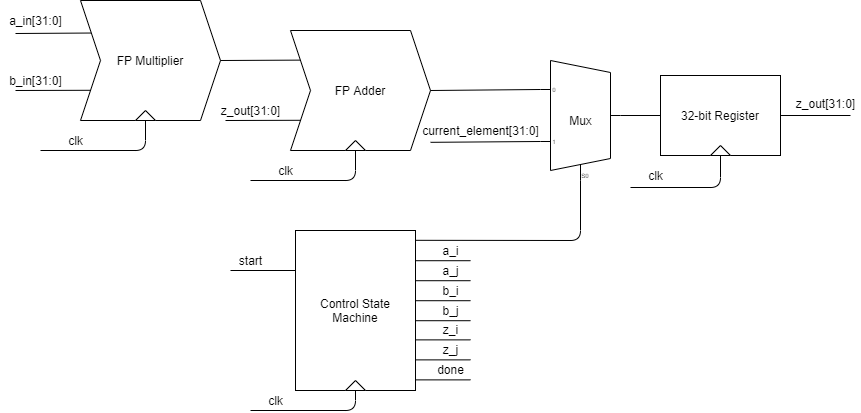
\includegraphics[width=1\linewidth]{Images/SequentialBD.png}
\caption{
\centering
بلوک دیاگرام ضرب‌کنندهٔ ماتریس ترتیبی.
}\label{fig:SequentialBD}
\end{figure}

زمان اجرای ضرب ماتریس در این ماژول،
$O(m^3)$
است. همچنین مساحت مورد استفاده
$O(1)$
است.

\subsection{
    ضرب‌کنندهٔ ماتریس سطری در ستونی
}

وظیفهٔ این ماژول، این است که با استفاده از یک ماژول ضرب‌کنندهٔ ماتریس ترتیبی، حاصل‌ضرب یک ماتریس سطری
$m \times n$
در یک ماتریس ستونی
$n \times m$
را محاسبه‌کند.
حاصل این ضرب، یک ماتریس
$m \times m$
خواهد بود.
\\
برای انجام این‌ کار، ابتدا ماتریس 
$m \times n$
به 
${\lceil\frac{n}{m}\rceil}$
ماتریس 
$m \times m$
تقسیم‌بندی می‌شود.
مشابهاً ماتریس 
$n \times m$
نیز به 
$\lceil\frac{n}{m}\rceil$
ماتریس 
$m \times m$
تقسیم‌بندی می‌شود.
حال با استفاده از ماژول ضرب‌کننده ماتریس ترتیبی و با توجه به این که قاعده ضرب بلوکی در ماتریس‌ها برقرار است، هر یک از این ماتریس‌های 
$m \times m$
به مانند یک عدد در نظر گرفته می‌شود و ماتریس‌های متناظر به ترتیب در هم ضرب می‌شوند.

شکل
\ref{fig:RowColBD}
بلوک دیاگرام ضرب‌کنندهٔ ماتریس سطری در ستونی است.
اندیس‌های
$a_i$
و
$b_j$
مستقیماً از ضرب‌کنندهٔ ماتریس ترتیبی حاصل می‌شوند، اما دیگر اندیس‌ها بصورت
\begin{align*}
    a_j &= mk + a_{j_{\text{seq}}}\\
    b_i &= mk + b_{i_{\text{seq}}}
\end{align*}
محاسبه می‌شوند، که در آن،
$k$
مشخص می‌کند که چندمین ماتریس
$m \times m$
در هر لحظه در حال محاسبه ضرب است، و
$a_{j_{\text{seq}}}$
و
$b_{i_{\text{seq}}}$
اندیس‌هایی هستند که ضرب‌کنندهٔ ماتریس ترتیبی تعیین کرده‌است.

\begin{figure}[t]
\centering 
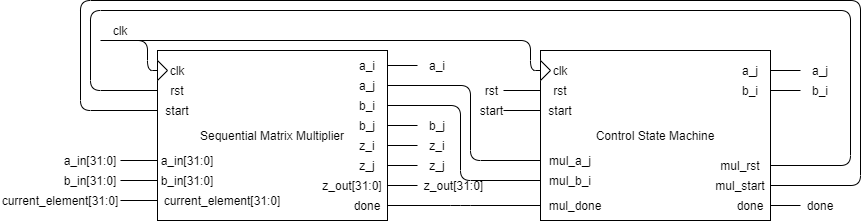
\includegraphics[width=1\linewidth]{Images/RowColBD.png}
\caption{
\centering
بلوک دیاگرام ضرب‌کنندهٔ ماتریس سطری در ستونی.
}\label{fig:RowColBD}
\end{figure}

زمان اجرای ضرب ماتریس در این ماژول،
$O(nm^2)$
است. همچنین از آنجایی که در این ماژول صرفا از یک ضرب‌کنندهٔ ترتیبی استفاده شده‌است، مساحت مورد استفاده
$O(1)$
است.

\subsection{
    ضرب‌کنندهٔ ماتریس موازی
}


این ماژول دو ماتریس 
$n \times n$
را به صورت موازی در هم ضرب می‌کند. 
به این صورت که ابتدا این ماتریس، به 
$\lceil\frac{n}{m}\rceil^2$
ماتریس 
$m \times m$
تقسیم‌بندی می‌شود.
سپس مطابق شکل
\ref{fig:ParallelMatrix}،
هر بلوک
$m \times m$
از ماتریس حاصل‌ضرب، توسط یک ضرب‌کنندهٔ ماتریس سطری در ستونی، بصورت موازی با دیگر بلوک‌های حاصل‌ضرب، محاسبه می‌شود.
در نتیجه، در این لایه، به تعداد
$\lceil\frac{n}{m}\rceil^2$،
ضرب‌کنندهٔ ماتریس سطری در ستونی ساخته می‌شود.
\begin{figure}[t]
\centering
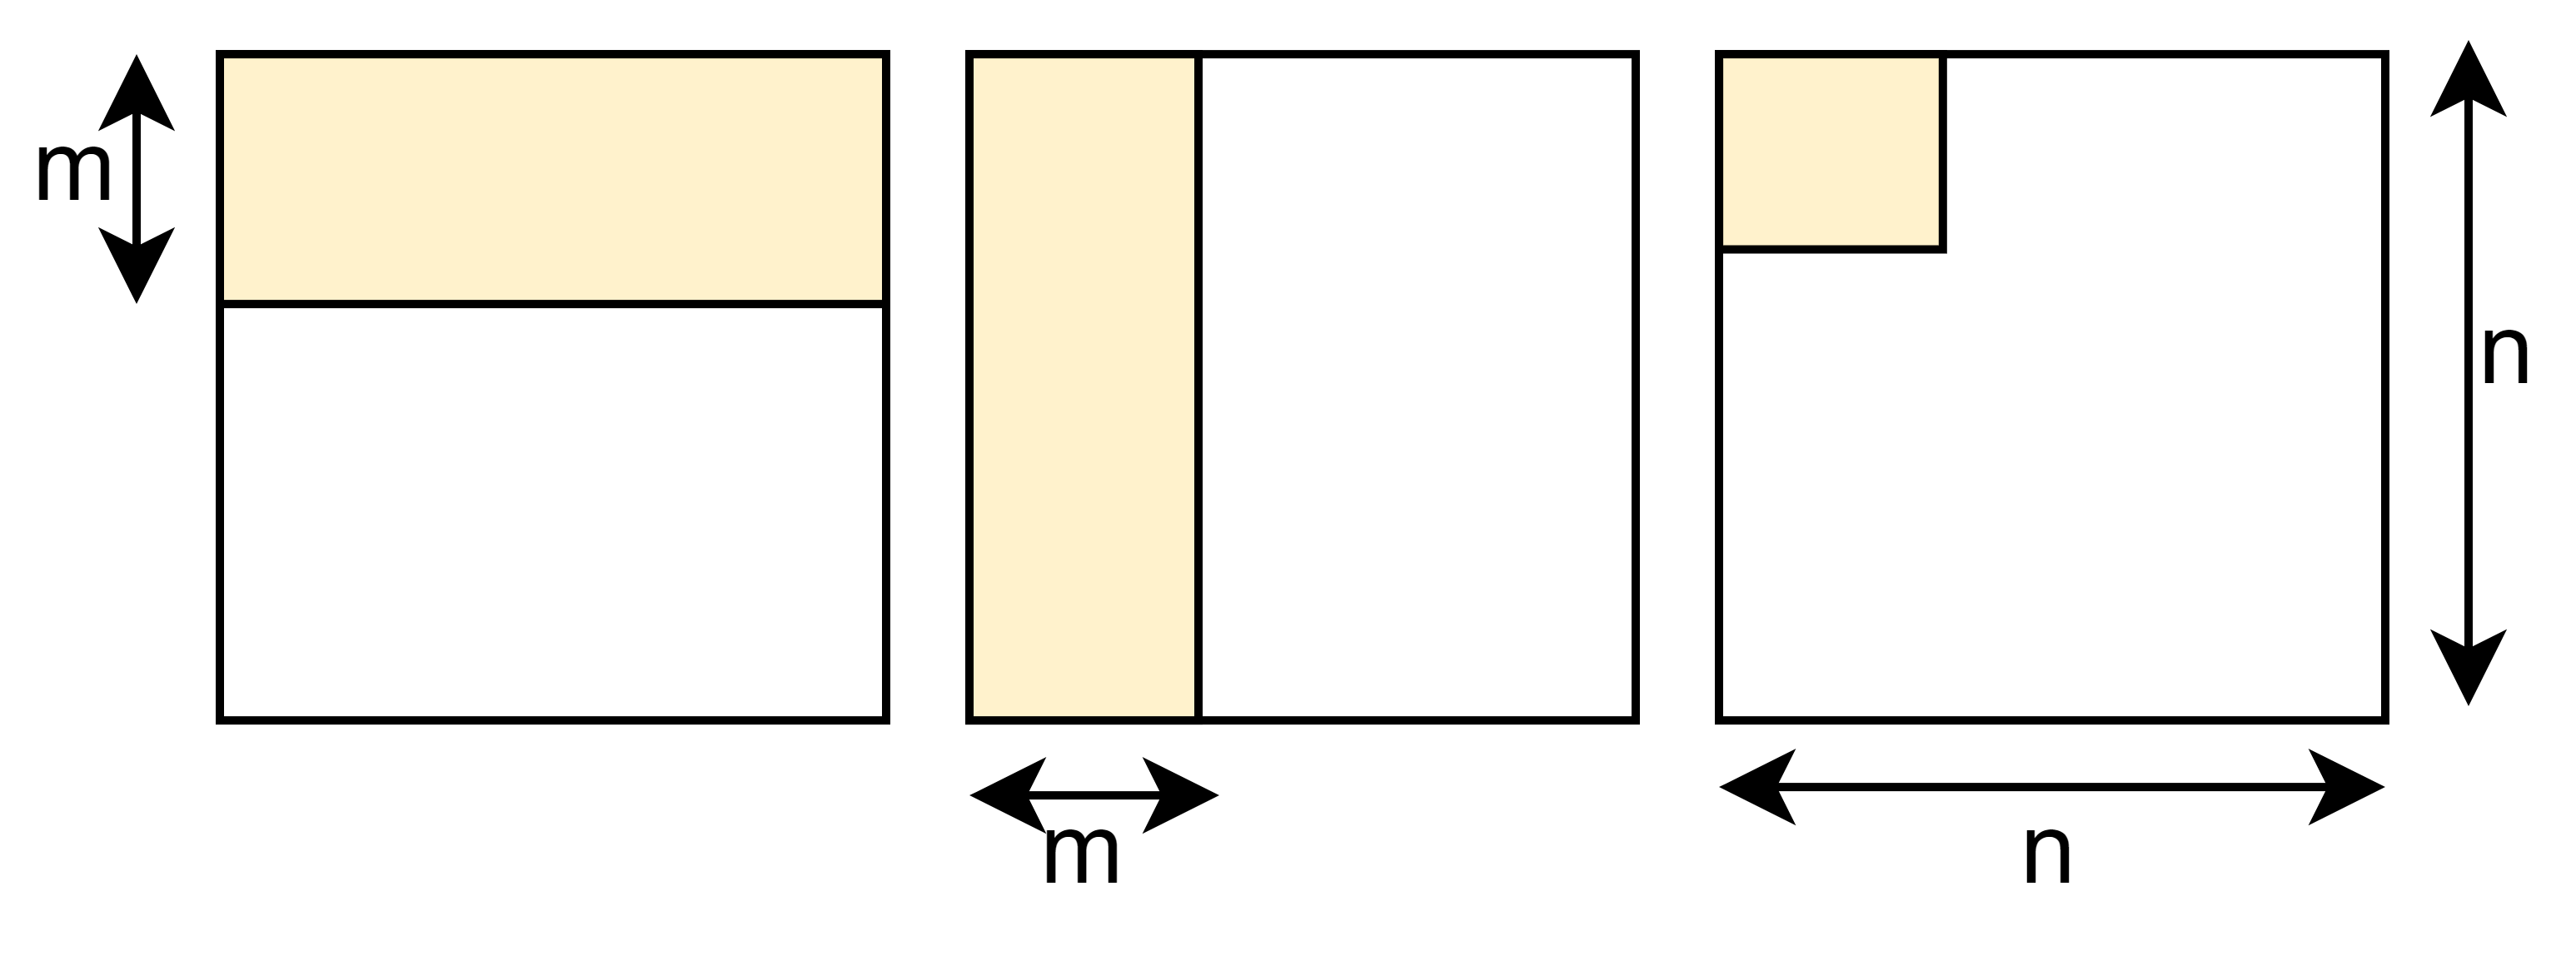
\includegraphics[width=1\linewidth]{Images/ParallelMatrix.png}
\caption{
\centering
روش محاسبهٔ حاصل‌ضرب یک بلوک از ماتریس جواب، توسط یک ضرب‌کنندهٔ ماتریس سطری در ستونی.
}\label{fig:ParallelMatrix}
\end{figure}

\begin{figure}[t]
\centering 
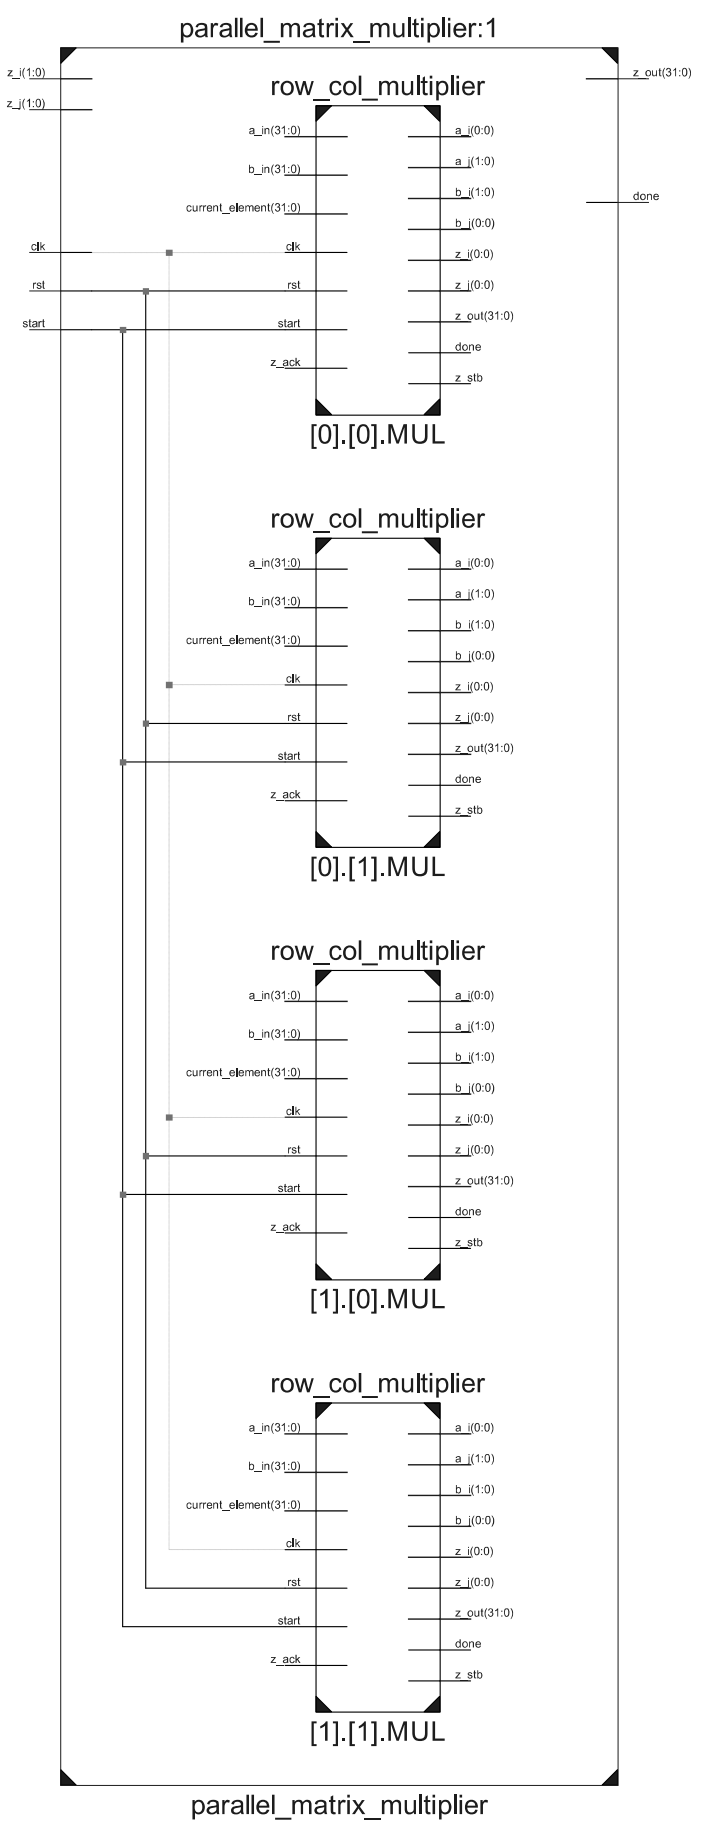
\includegraphics[width=.8\linewidth]{Images/ParallelBD.png}
\caption{
\centering
بلوک دیاگرام ضرب‌کنندهٔ ماتریس موازی.
}\label{fig:ParallelBD}
\end{figure}

شکل
\ref{fig:ParallelBD}
بلوک دیاگرام ضرب‌کنندهٔ ماتریس موازی را نمایش می‌دهد.
حافظهٔ ماتریس‌های ورودی و خروجی در این ماژول موجود است، اما به علت پیچیدگی اتصالات مربوط به این حافظه‌ها، از نمایش آن‌ها در بلوک دیاگرام صرف نظر شده‌است. 

\begin{figure}[t]
\centering 
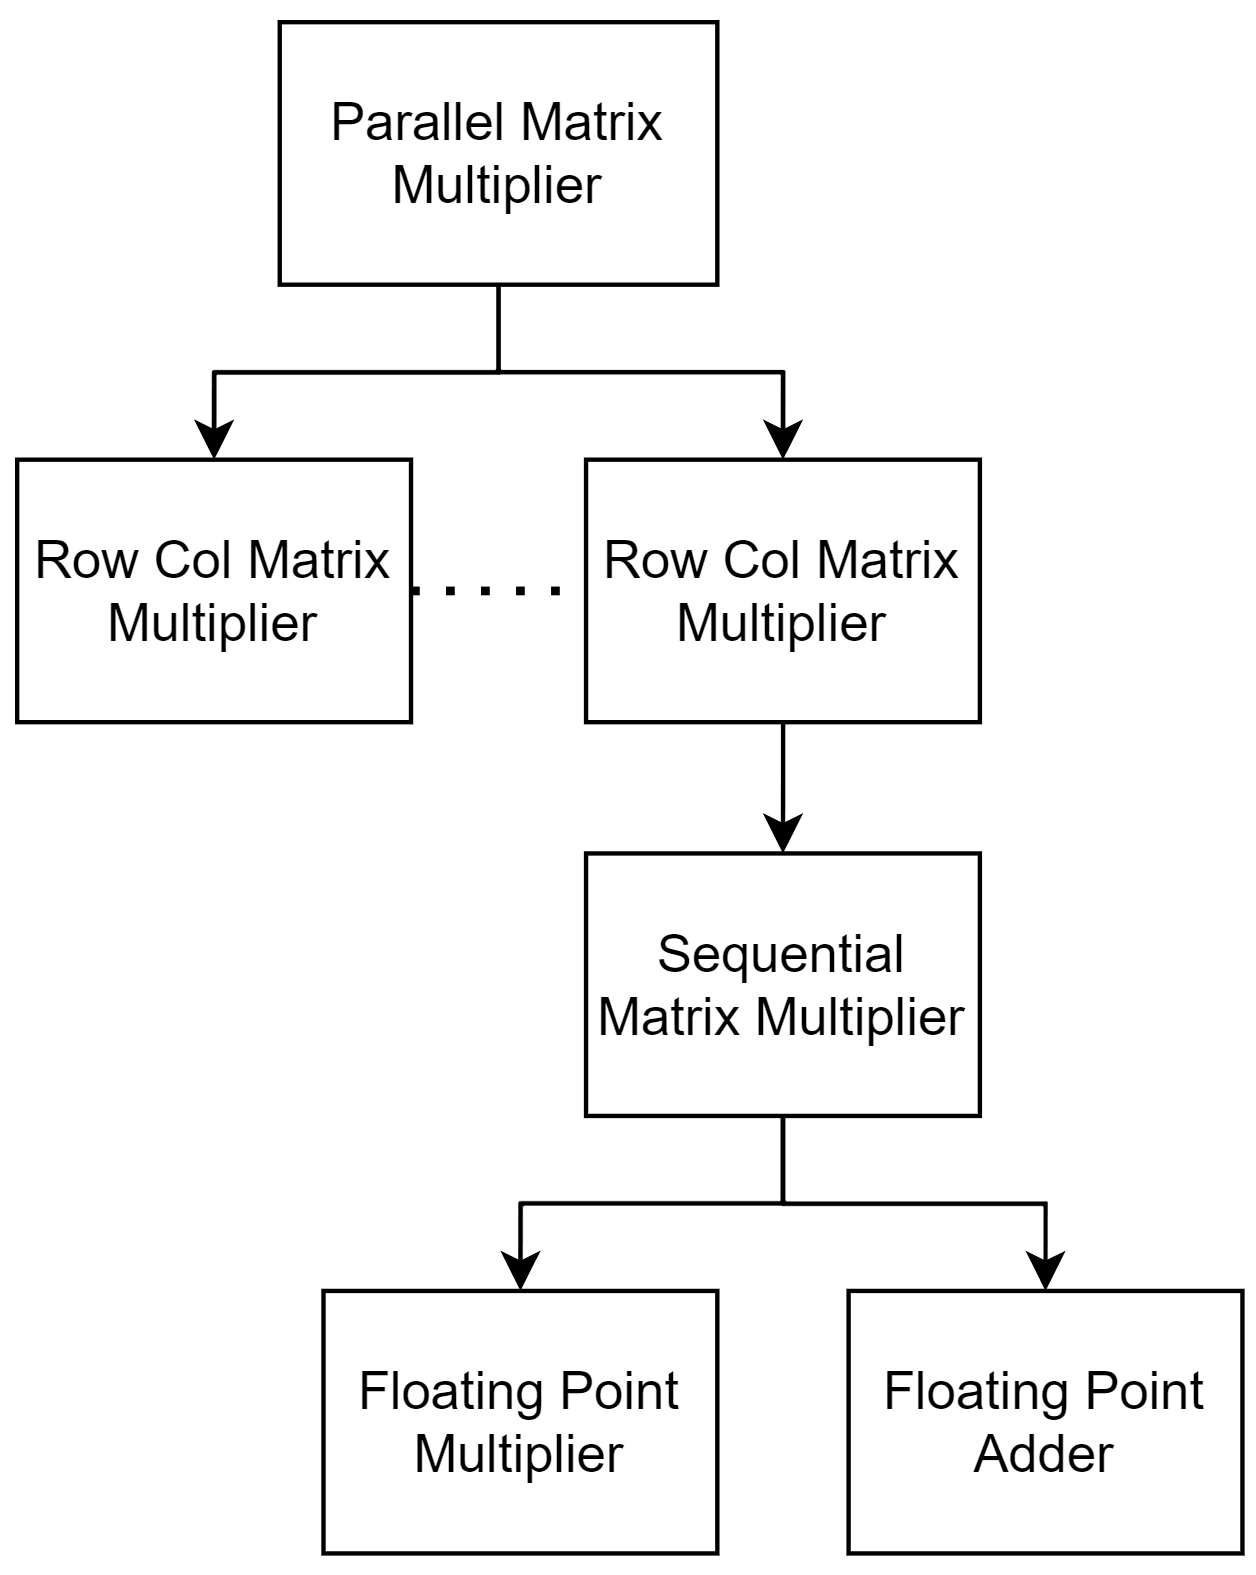
\includegraphics[width=\linewidth]{Images/HierarchicalTree.png}
\caption{
\centering
ساختار درختی سیستم.
}\label{fig:HierarchicalTree}
\end{figure}

زمان اجرای ضرب ماتریس در این ماژول، معادل زمان اجرای یک ضرب‌کنندهٔ سطری در ستونی است که برابر
$O(nm^2)$
است. همچنین از آنجایی که در این ماژول از 
$(\frac{n}{m})^2$
ماژول ضرب‌کنندهٔ سطری در ستونی استفاده شده‌است، مساحت مورد استفاده
$O((\frac{n}{m})^2)$
است.

در نهایت، ساختار درختی کل سیستم در شکل
\ref{fig:HierarchicalTree}
نمایش داده‌شده است.

\section{شبیه‌سازی و نتایج}

برای هر یک از ماژول‌های شرح داده شده در بخش قبل، یک
\lr{Testbench}
نوشته شده‌است.
مقادیر ورودی، در قالب فایل‌های باینری در پوشهٔ
\lr{data}
موجود اند و در ابتدای اجرای شبیه‌سازی، از فایل‌های مربوطه خوانده شده و در حافظه نوشته می‌شوند.
همچنین پس از اجرای عملیات ضرب ماتریس، خروجی حاصل در فایل
\lr{sim\_out.bin}
نوشته می‌شود.

برای بررسی و مقایسهٔ پاسخ‌های حاصل از شبیه‌سازی، یک مدل طلایی توسط زبان پایتون نوشته شده‌است
که ورودی‌ها و خروجی حاصل از شبیه‌سازی را دریافت کرده، و پاسخ صحیح را با پاسخ به دست آمده مقایسه می‌کند.
اجرای مدل طلایی، توسط دستور زیر قابل انجام است.

\begin{latin}
\begin{lstlisting}
python gold_standard/model.py data/<input_a address> data/<input_b address> <sim_out.bin address> <n> <k> <m>
\end{lstlisting}
\end{latin}

در ادامه به هر کدام از
\lr{Testbench}ها
به تفصیل پرداخته می‌شود.

\subsection{
    ضرب‌کنندهٔ ماتریس ترتیبی
}

برای آزمایش و شبیه‌سازی این ماژول، دو ماتریس
$4 \times 4$
به صورت زیر در هم ضرب شدند.

\tiny
\begin{align}
    \left[
        \begin{array}{c c c c}
            1&2&3&4\\
            5&6&7&8\\
            9&10&11&12\\
            13&14&15&16
        \end{array}
    \right] . \left[
        \begin{array}{c c c c}
            2&0&0&0\\
            0&2&0&0\\
            0&0&2&0\\
            0&0&0&2
        \end{array}
    \right]
    = \left[
        \begin{array}{c c c c}
            2&4&6&8\\
            10&12&14&16\\
            18&20&22&24\\
            26&28&30&32
        \end{array}
    \right]
    \label{eq:SquareMatrix}
\end{align}
\normalsize

در این
\lr{Testbench}،
ابتدا ورودی‌ها از فایل‌های مربوطه خوانده شده، سپس سیگنال
\lr{start}
مربوط به ضرب‌کنندهٔ ماتریس ترتیبی فعال می‌شود. پس از فعال شدن سیگنال
\lr{done}
در ماژول ضرب‌کننده، نتیجهٔ حاصل در فایل خروجی نوشته می‌شود.
نتیجهٔ اجرای مدل طلایی نیز بصورت زیر است.

\begin{latin}
\begin{lstlisting}[language=Bash]
> python .\gold_standard\model.py .\data\square_input_a.bin .\data\square_input_b.bin .\sim_out.bin 4 4 4
A:
[[ 1.  2.  3.  4.]
[ 5.  6.  7.  8.]
[ 9. 10. 11. 12.]
[13. 14. 15. 16.]]
B:
[[2. 0. 0. 0.]
[0. 2. 0. 0.]
[0. 0. 2. 0.]
[0. 0. 0. 2.]]
Actual:
[[ 2.  4.  6.  8.]
[10. 12. 14. 16.]
[18. 20. 22. 24.]
[26. 28. 30. 32.]]
Expected:
[[ 2.  4.  6.  8.]
[10. 12. 14. 16.]
[18. 20. 22. 24.]
[26. 28. 30. 32.]]
True
\end{lstlisting}
\end{latin}

\subsection{
    ضرب‌کنندهٔ ماتریس سطری در ستونی
}

برای آزمایش و شبیه‌سازی این ماژول، دو ماتریس
$4 \times 8$
و
$8 \times 4$
به صورت زیر در هم ضرب شدند.

\scriptsize
\begin{align*}
    &A \times B\\
    &=\left[
        \begin{array}{c c c c c c c c}
            1&2&3&4&5&6&7&8\\
            1&2&3&4&5&6&7&8\\
            1&2&3&4&5&6&7&8\\
            1&2&3&4&5&6&7&8
        \end{array}
    \right] . \left[
        \begin{array}{c c c c}
            1.5&0&0&0\\
            0&1.5&0&0\\
            0&0&1.5&0\\
            0&0&0&1.5\\
            1.5&0&0&0\\
            0&1.5&0&0\\
            0&0&1.5&0\\
            0&0&0&1.5
        \end{array}
    \right]\\
    &= \left[
        \begin{array}{c c c c}
            9&12&15&18\\
            9&12&15&18\\
            9&12&15&18\\
            9&12&15&18
        \end{array}
    \right]
\end{align*}
\normalsize

در این
\lr{Testbench}،
ابتدا ورودی‌ها از فایل‌های مربوطه خوانده شده، سپس سیگنال
\lr{start}
مربوط به ضرب‌کنندهٔ ماتریس ترتیبی فعال می‌شود. پس از فعال شدن سیگنال
\lr{done}
در ماژول ضرب‌کننده، نتیجهٔ حاصل در فایل خروجی نوشته می‌شود.
نتیجهٔ اجرای مدل طلایی نیز بصورت زیر است.

\begin{latin}
\begin{lstlisting}[language=Bash]
> python .\gold_standard\model.py .\data\row_input.bin .\data\col_input.bin .\sim_out.bin 4 8 4
A:
[[1. 2. 3. 4. 5. 6. 7. 8.]
[1. 2. 3. 4. 5. 6. 7. 8.]
[1. 2. 3. 4. 5. 6. 7. 8.]
[1. 2. 3. 4. 5. 6. 7. 8.]]
B:
[[1.5 0.  0.  0. ]
[0.  1.5 0.  0. ]
[0.  0.  1.5 0. ]
[0.  0.  0.  1.5]
[1.5 0.  0.  0. ]
[0.  1.5 0.  0. ]
[0.  0.  1.5 0. ]
[0.  0.  0.  1.5]]
Actual:
[[ 9. 12. 15. 18.]
[ 9. 12. 15. 18.]
[ 9. 12. 15. 18.]
[ 9. 12. 15. 18.]]
Expected:
[[ 9. 12. 15. 18.]
[ 9. 12. 15. 18.]
[ 9. 12. 15. 18.]
[ 9. 12. 15. 18.]]
True
\end{lstlisting}
\end{latin}
\subsection{
    ضرب‌کنندهٔ ماتریس موازی
}
برای آزمایش و شبیه‌سازی این ماژول، همان دو ماتریس
رابطه 
\ref{eq:SquareMatrix}
در هم ضرب شده‌اند. اما تفاوت در این‌جا این است که در این حالت هر یک از ماتریس‌ها، به چهار ماتریس 
$2 \times 2$
تقسیم شده‌اند.
($m = 2$)


در این
\lr{Testbench}،
ابتدا ورودی‌ها از فایل‌های مربوطه خوانده شده، سپس سیگنال
\lr{start}
مربوط به ضرب‌کنندهٔ ماتریس ترتیبی فعال می‌شود. پس از فعال شدن سیگنال
\lr{done}
در ماژول ضرب‌کننده، نتیجهٔ حاصل در فایل خروجی نوشته می‌شود.
نتیجهٔ اجرای مدل طلایی نیز بصورت زیر است.

\begin{latin}
\begin{lstlisting}[language=Bash]
> python .\gold_standard\model.py .\data\square_input_a.bin .\data\square_input_b.bin .\sim_out.bin 4 4 4
A:
[[ 1.  2.  3.  4.]
[ 5.  6.  7.  8.]
[ 9. 10. 11. 12.]
[13. 14. 15. 16.]]
B:
[[2. 0. 0. 0.]
[0. 2. 0. 0.]
[0. 0. 2. 0.]
[0. 0. 0. 2.]]
Actual:
[[ 2.  4.  6.  8.]
[10. 12. 14. 16.]
[18. 20. 22. 24.]
[26. 28. 30. 32.]]
Expected:
[[ 2.  4.  6.  8.]
[10. 12. 14. 16.]
[18. 20. 22. 24.]
[26. 28. 30. 32.]]
True
\end{lstlisting}
\end{latin}
شکل موج‌ها
\LTRfootnote{\lr{waveforms}} 
در بخش ضمیمه‌ها نمایش داده شده‌است.

\section{سنتز بر روی
\lr{FPGA}
و نتایج}

\begin{figure}[t]
\centering
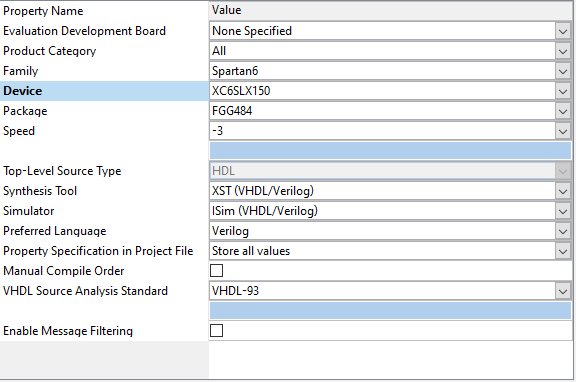
\includegraphics[width=\linewidth]{Images/FPGASettings.png}
\caption{
\centering
تنظیمات
\lr{FPGA}.
}\label{fig:FPGASettings}
\end{figure}

با استفاده از نرم‌افزار
\lr{XilinxISE}،
پروژه‌ای برای یک
\lr{FPGA}
با تنظیماتی که در شکل
\ref{fig:FPGASettings}
نمایش داده‌شده است، ساخته شد.
سپس فایل‌های
\lr{FP\_adder.v}،
\lr{FP\_multiplier.v}،
\lr{sequential\_matrix\_multipiler.v}،
\lr{row\_col\_multiplier.v}
و
\lr{parallel\_matrix\_multiplier.v} 
به
\lr{sources}
پروژه اضافه شد و
ماژول
\lr{parallel\_matrix\_multiplier}
به عنوان
\lr{System Top}
در نظر گرفته شد. پس از تعیین منابع پروژه،
\lr{System Top}
سنتز شد. در این سنتز، مقدار پارامتر
$n$
برابر ۴ و
$m$
برابر ۲ در نظر گرفته شد.

\begin{latin}
\begin{table}[t]
\centering
\scriptsize
\caption{\lr{Device Utilization Summary (estimated values).}}
\begin{tabular}[t]{|l|l|c|c|c|}
\hline
\multicolumn{2}{|l|}{Logic Utilization}                 & Used       & Available       & Utilization       \\ \hline
\multicolumn{2}{|l|}{Number of Slice Registers}         & 2932       & 184304          & 1\%               \\ \hline
\multicolumn{2}{|l|}{Number of Slice LUTs}              & 4508       & 92152           & 4\%               \\ \hline
\multicolumn{2}{|l|}{Number of fully used LUT-FF pairs} & 2261       & 5179            & 43\%              \\ \hline
\multicolumn{2}{|l|}{Number of bonded IOBs}             & 40         & 338             & 11\%              \\ \hline
\multicolumn{2}{|l|}{Number of BUFG/BUFGCTRLs}          & 1          & 16              & 6\%               \\ \hline
\multicolumn{2}{|l|}{Number of DSP48A1s}                & 16         & 180             & 8\%               \\ \hline
\end{tabular}
\label{tab:DeviceUtilSummary}
\end{table}
\end{latin}

در جدول
\ref{tab:DeviceUtilSummary}
مقدار استفاده از بخش‌های مختلف
\lr{FPGA}
که توسط ابزار سنتز بدست آمده‌است، نشان داده شده است. گزارش زمانی سنتز نیز بصورت زیر می‌باشد.

\begin{latin}
\begin{lstlisting}
Timing Summary:
---------------
Speed Grade: -3

Minimum period: 15.993ns (Maximum Frequency: 62.528MHz)
Minimum input arrival time before clock: 2.762ns
Maximum output required time after clock: 5.694ns
Maximum combinational path delay: 7.920ns
\end{lstlisting}
\end{latin}

خروجی‌های مربوط به سنتز، در پوشهٔ
\lr{synthesis}
موجود است.

\section{نتیجه‌گیری}
در این پروژه به طراحی، پیاده سازی، شبیه سازی و سنتز یک ضرب‌کننده ماتریسی پرداخته شد. 
ساختار این ضرب‌کننده از چند لایه مختلف تشکیل شده است که مهم‌ترین آن‌ها دو لایه هستند. لایه اصلی اول،  ضرب‌کننده ماتریس ترتیبی
است که مانند الگوریتم رایج ضرب ماتریس‌‌ها، حاصلضرب را به صورت ترتیبی محاسبه می‌کند. 
لایه اصلی دوم، ضرب‌کننده ماتریس موازی است که با شکاندن ماتریس به زیر-ماتریس ‌‌های کوچکتر، فرایند ضرب ماتریسی را تا 
حدی به صورت موازی انجام می‌دهد.\\
ویژگی خوب این طراحی این است که می‌توان با تناسب مقادیر
$m$
و
$n$،
تعادلی بین زمان اجرای ضرب ماتریسی و میزان سخت‌افزار مصرف شده به وجود آورد. به این صورت که به ازای 
$n$
ثابت، هر چه
$m$
بزرگتر باشد، عملیات ضرب به سمت کاملا ترتیبی شدن پیش می‌رود، و هرچه
$m$
کوچکتر باشد میزان موازی‌سازی بیشتر می‌شود. در نتیجه،‌ هرچه میزان موازی‌سازی بیشتر شود، مساحت مورد استفاده افزایش می‌یابد، اما سرعت اجرا نیز بیشتر می‌شود.\\
 همچنین در نهایت عملیات سنتز انجام شد و مقادیر میزان استفاده از 
 \lr{FPGA}
 نیز محاسبه و گزارش شدند. بیشترین میزان فرکانس مدار نیز برابر 
 $62.528 MH$
 است.

\newpage
\onecolumn

\section{ضمیمه‌ها}

\begin{figure}[ht]
\centering
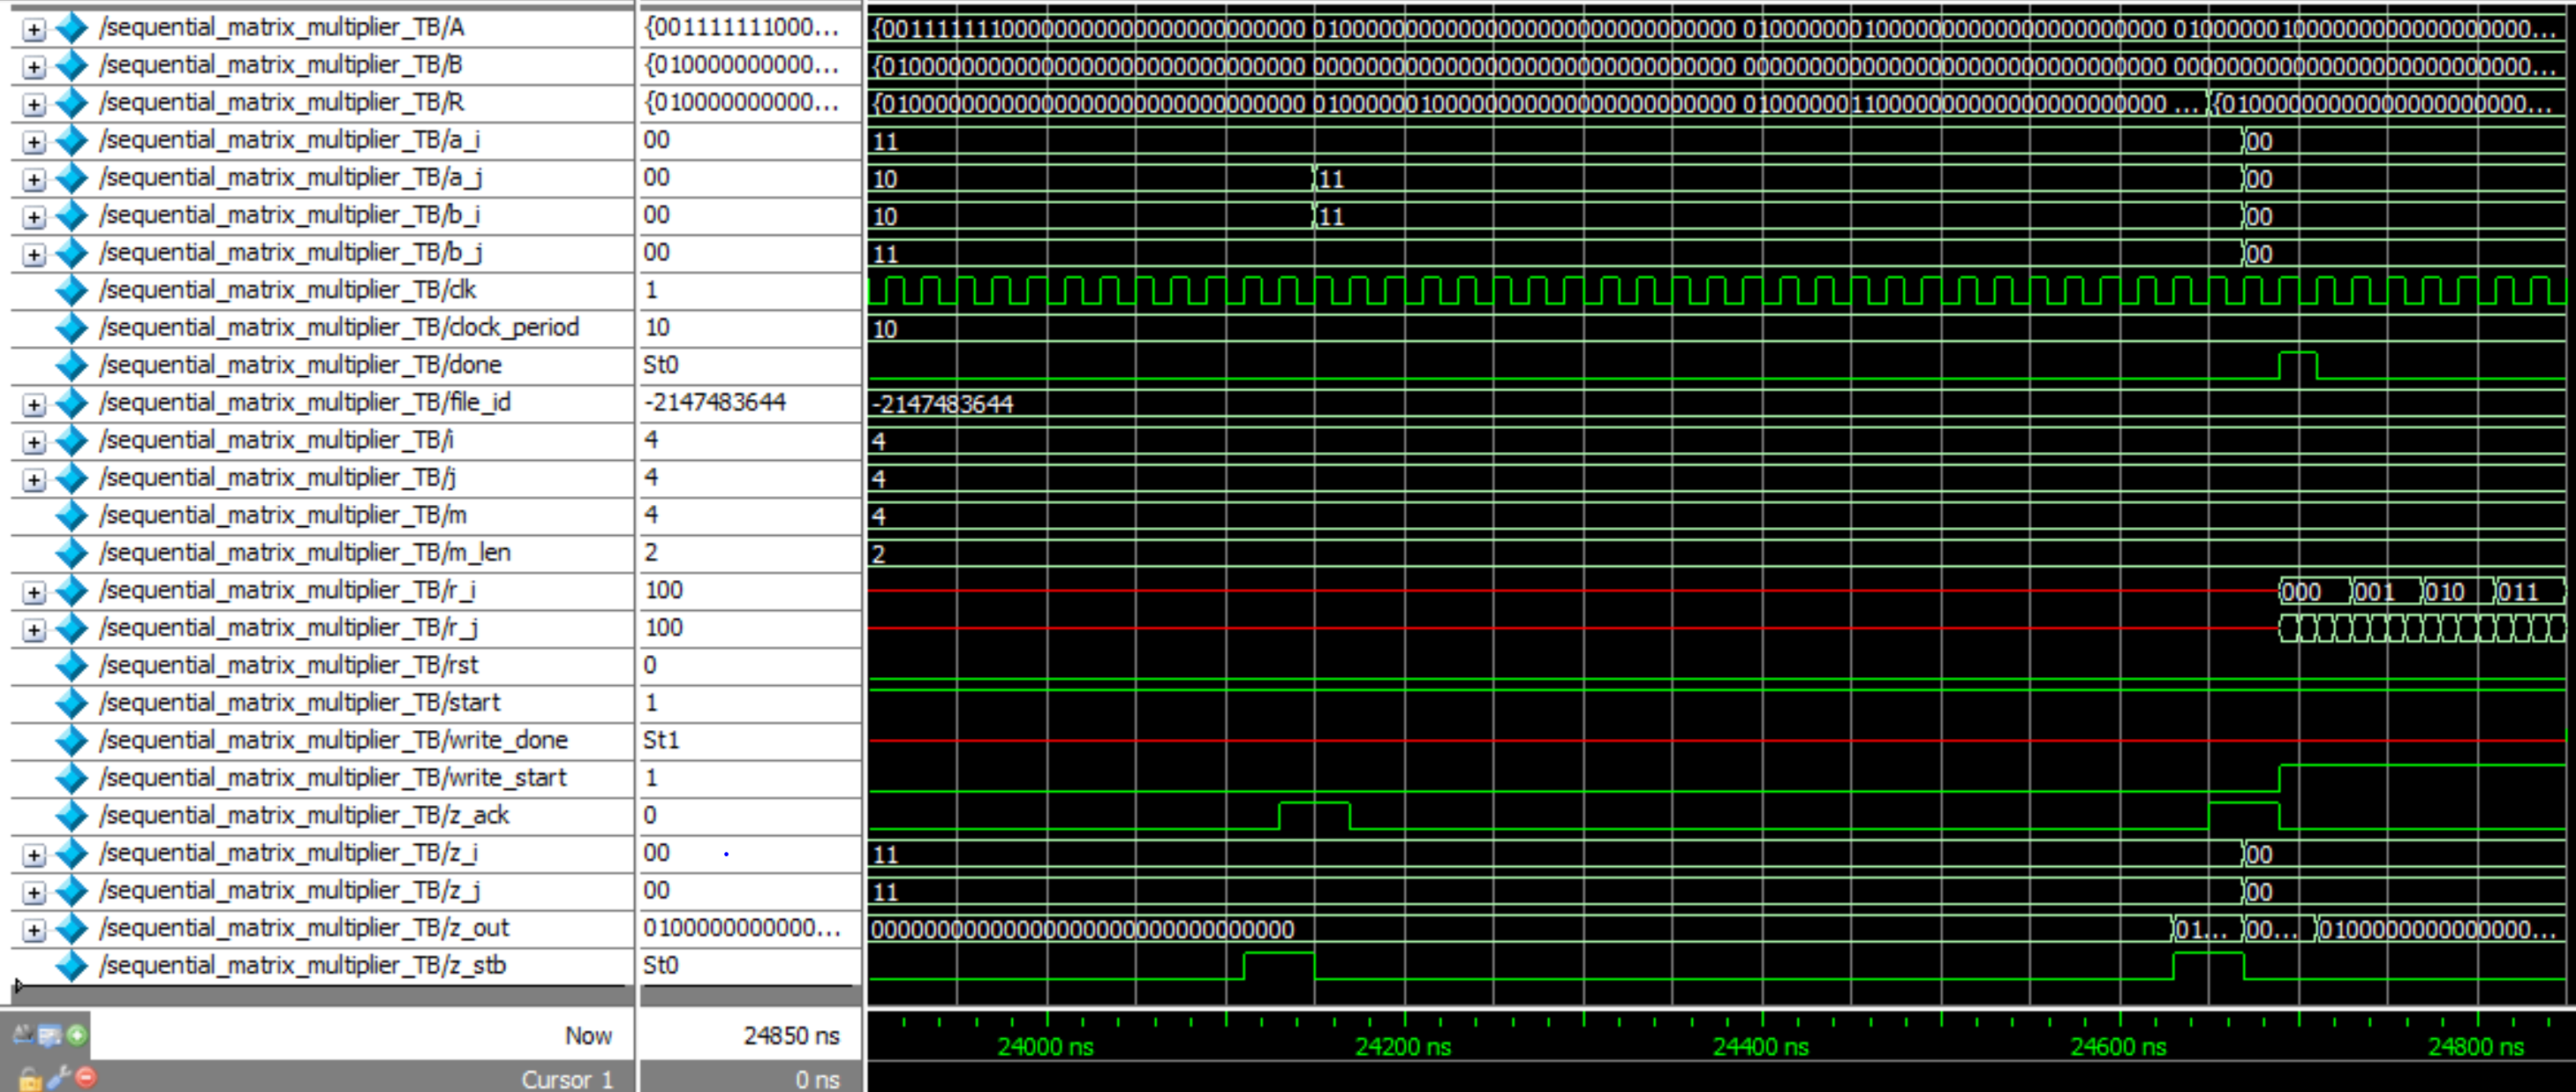
\includegraphics[width=.85\linewidth]{Images/SequentialWF.png}
\caption{
\centering
شکل موج شبیه‌سازی ماژول ضرب‌کننده ماتریس ترتیبی
}
\end{figure}

\begin{figure}[ht]
\centering
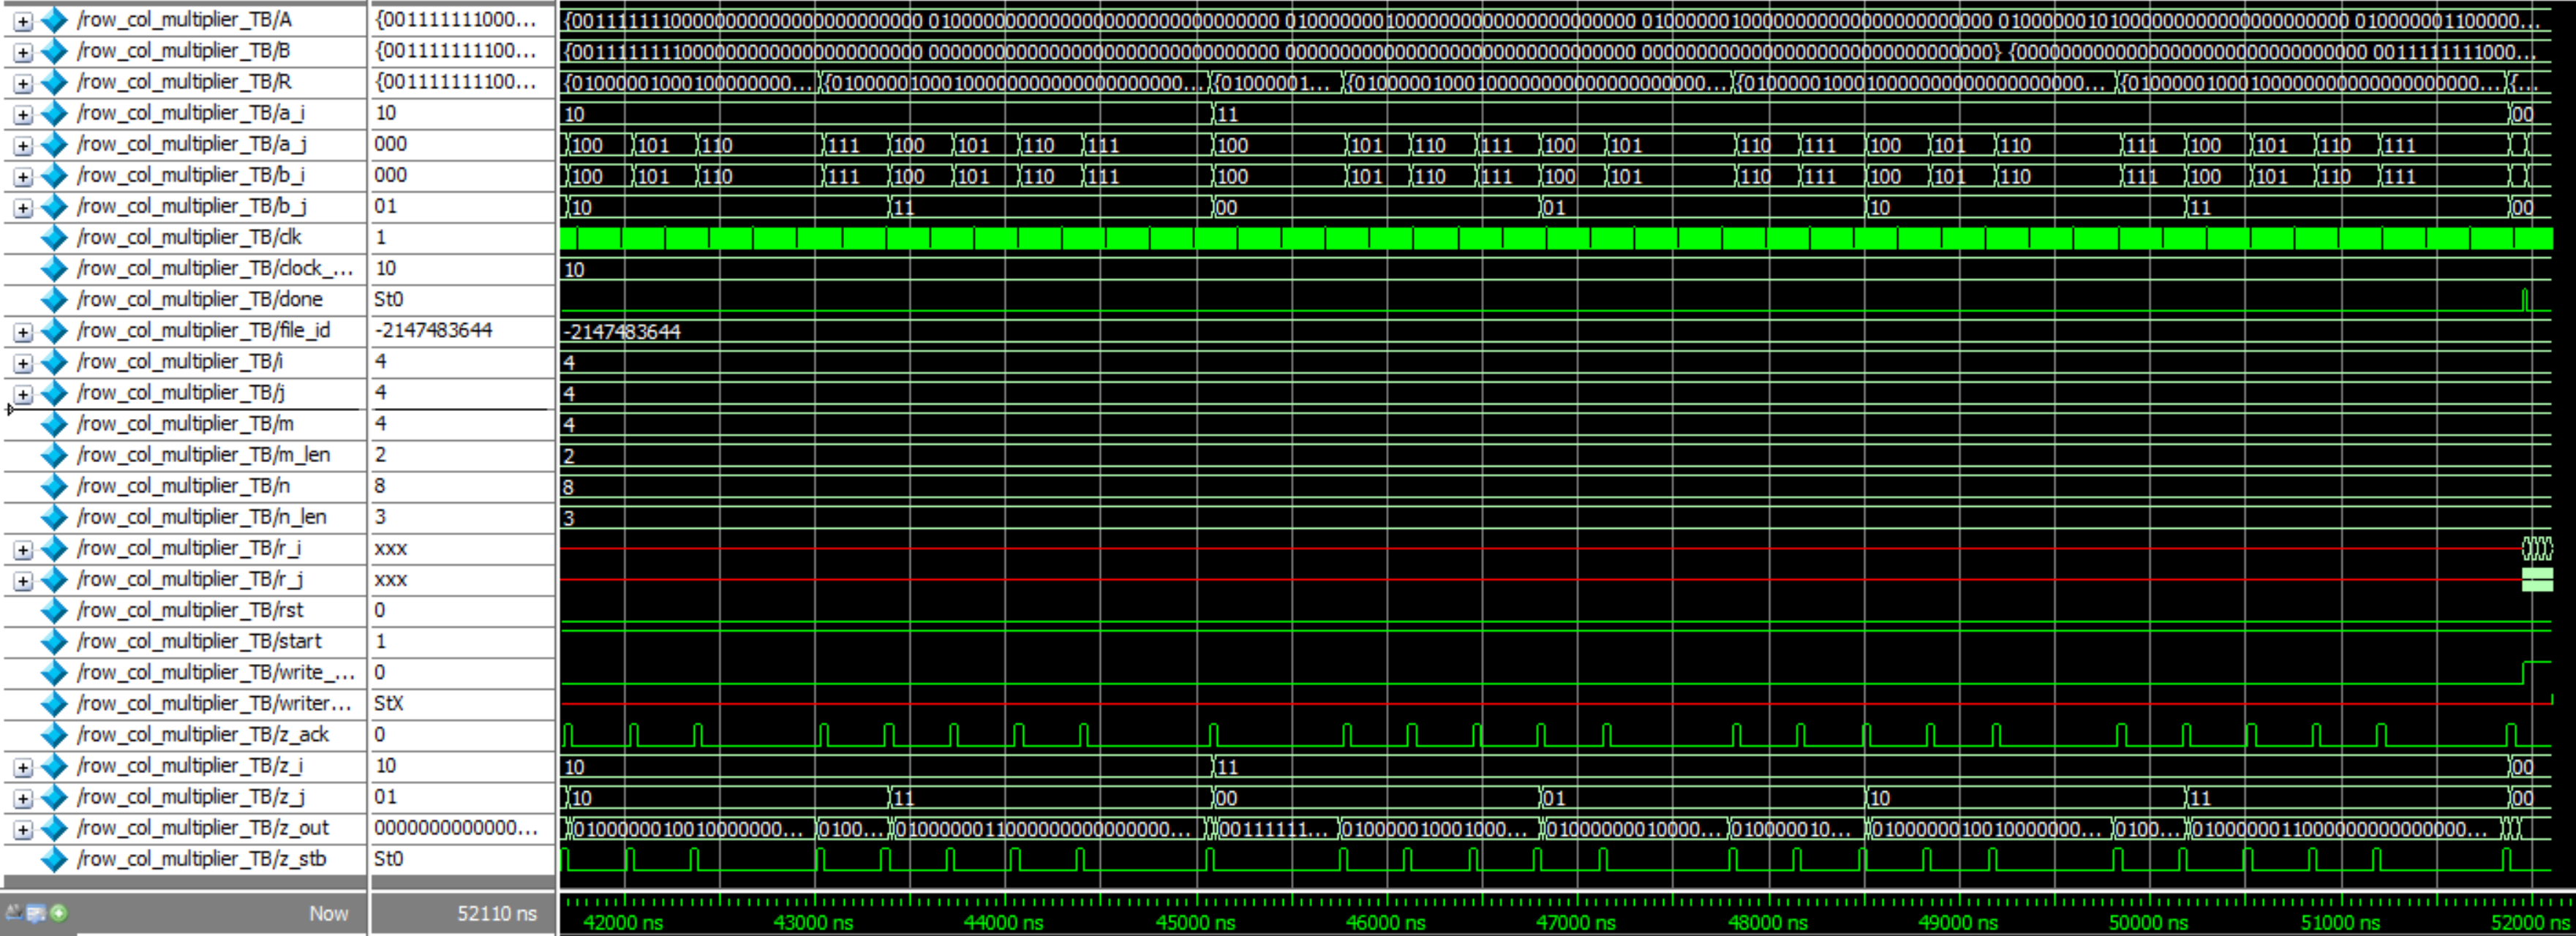
\includegraphics[width=.85\linewidth]{Images/RowColWF.png}
\caption{
\centering
شکل موج شبیه‌سازی ماژول ضرب‌کننده ماتریس سطری در ستونی
}
\end{figure}

\begin{figure}[ht]
\centering
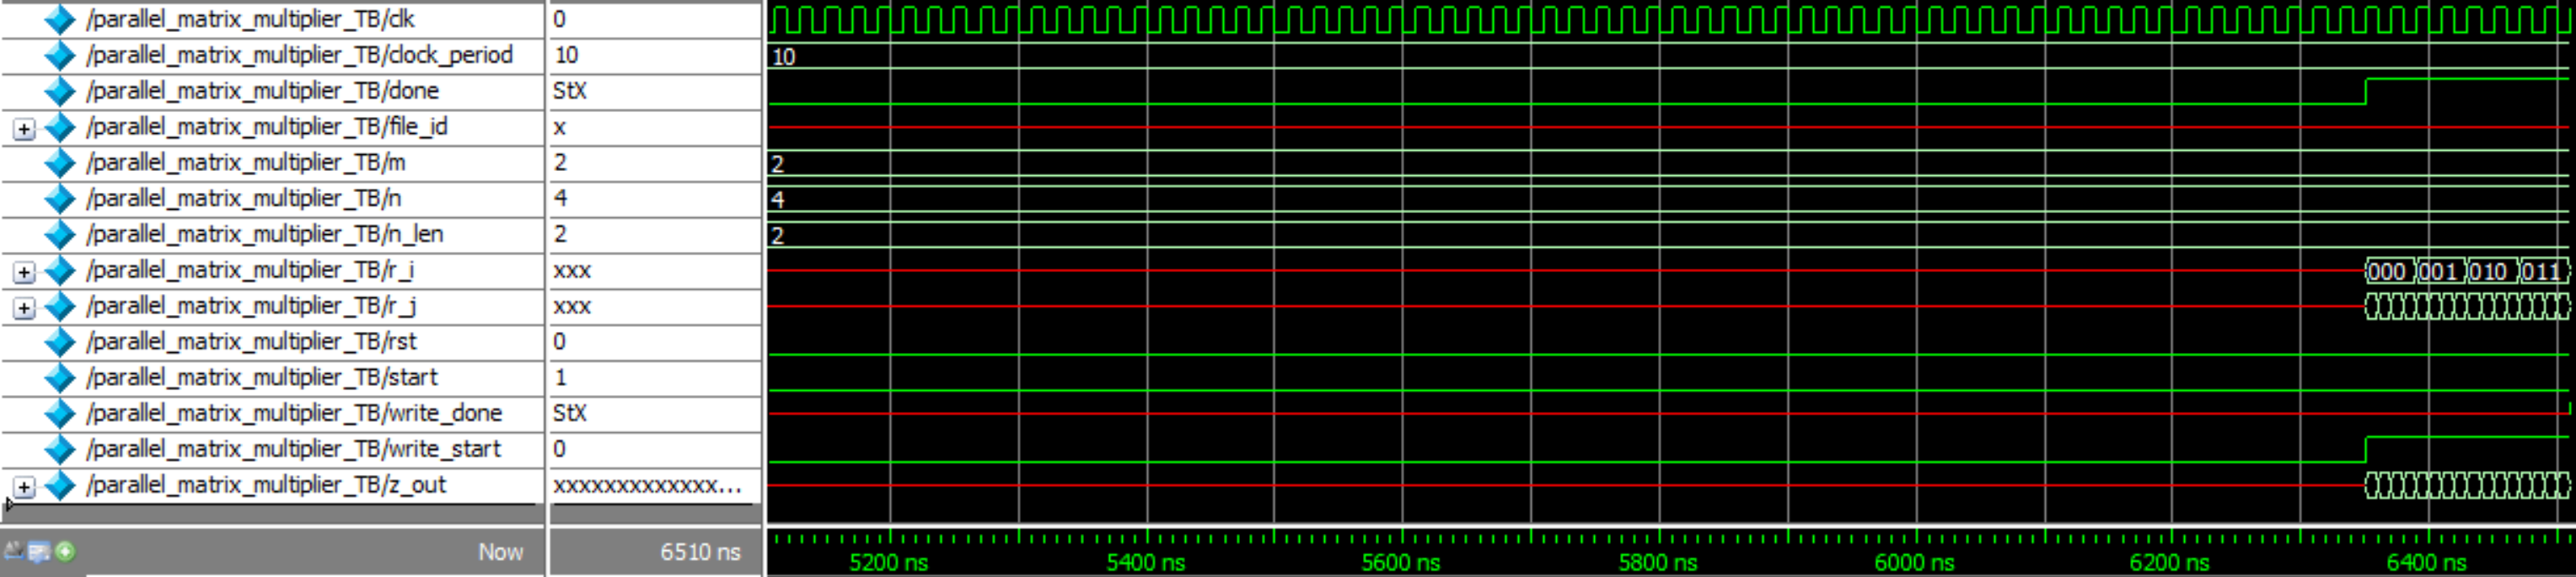
\includegraphics[width=.85\linewidth]{Images/ParallelWF.png}
\caption{
\centering
شکل موج شبیه‌سازی ماژول ضرب‌کننده ماتریس موازی
}
\end{figure}

\end{document}